\documentclass[a4paper,12pt,twoside]{memoir}

% Castellano
\usepackage[spanish,es-tabla]{babel}
\selectlanguage{spanish}
\usepackage[utf8]{inputenc}
\usepackage[T1]{fontenc}
\usepackage{lmodern} % scalable font
\usepackage{microtype}
\usepackage{placeins}
\usepackage{listings}
\usepackage[usenames,dvipsnames]{color}
\usepackage{textgreek}


\lstdefinestyle{mystyle}{
    backgroundcolor=\color[rgb]{0.95,0.95,0.92},
    breakatwhitespace=false,         
    breaklines=true,                 
    captionpos=b,                    
    keepspaces=true,                 
    numbers=left,                    
    numbersep=5pt,                  
    showspaces=false,                
    showstringspaces=false,
    showtabs=false,                  
    tabsize=2
}

\lstset{style=mystyle}




\usepackage[style=numeric,sorting=none]{biblatex} % Para la bibliografia
\addbibresource{bibliografiaAnexos.bib} % Para la bibliografia
\usepackage{geometry} 

\RequirePackage{booktabs}
\RequirePackage[table]{xcolor}
\RequirePackage{xtab}
\RequirePackage{multirow}

% Links
\PassOptionsToPackage{hyphens}{url}\usepackage[colorlinks]{hyperref}
\hypersetup{
	allcolors = {black} % Originalmente estaba en 'red'
}

% Ecuaciones
\usepackage{amsmath}

% Rutas de fichero / paquete
\newcommand{\ruta}[1]{{\sffamily #1}}

% Párrafos
\nonzeroparskip

% Huérfanas y viudas
\widowpenalty100000
\clubpenalty100000

% Evitar solapes en el header
\nouppercaseheads


\let\tmp\oddsidemargin
\let\oddsidemargin\evensidemargin
\let\evensidemargin\tmp
\reversemarginpar



% Imagenes
\usepackage{graphicx}
\newcommand{\imagen}[2]{
	\begin{figure}[!h]
		\centering
		\includegraphics[width=0.9\textwidth]{#1}
		\caption{#2}\label{fig:#1}
	\end{figure}
	\FloatBarrier
}






\graphicspath{ {./img/} }

% Capítulos
\chapterstyle{bianchi}
\newcommand{\capitulo}[2]{
	\setcounter{chapter}{#1}
	\setcounter{section}{0}
	\setcounter{figure}{0}
	\setcounter{table}{0}
	\chapter*{#2}
	\addcontentsline{toc}{chapter}{#2}
	\markboth{#2}{#2}
}

% Apéndices
\renewcommand{\appendixname}{Apéndice}
\renewcommand*\cftappendixname{\appendixname}

\newcommand{\apendice}[1]{
	%\renewcommand{\thechapter}{A}
	\chapter{#1}
}

\renewcommand*\cftappendixname{\appendixname\ }

% Formato de portada
\makeatletter
\usepackage{xcolor}
\newcommand{\tutor}[1]{\def\@tutor{#1}}
\newcommand{\tutorb}[1]{\def\@tutorb{#1}}
\newcommand{\course}[1]{\def\@course{#1}}
\definecolor{cpardoBox}{HTML}{E6E6FF}
\def\maketitle{
  \null
  \thispagestyle{empty}
  % Cabecera ----------------
\begin{center}
  \noindent
\includegraphics[width=\textwidth]{cabeceraSalud}\vspace{1.5cm}%
\end{center}
  
  % Título proyecto y escudo salud ----------------
  \begin{center}
    \begin{minipage}[c][1.5cm][c]{.20\textwidth}
        
\includegraphics[width=\textwidth]{escudoSalud.pdf}
    \end{minipage}
  \end{center}
  
  \begin{center}
    \colorbox{cpardoBox}{%
        \begin{minipage}{.8\textwidth}
          \vspace{.5cm}\Large
          \begin{center}
          \textbf{TFG del Grado en Ingeniería de la Salud}\vspace{.6cm}\\
          \textbf{\LARGE\@title{}}
          \end{center}
          \vspace{.2cm}
        \end{minipage}
    }%
  \end{center}
  
    % Datos de alumno, curso y tutores ------------------
  \begin{center}%
  {%
    \noindent\LARGE
    Presentado por \@author{}\\ 
    en la Universidad de Burgos\\
    \vspace{0.5cm}
    \noindent\Large
    \@date{}\\
    \vspace{0.5cm}
    Tutor: \@tutor{}\\ % comenta el que no corresponda
    %Tutores: \@tutor{} -- \@tutorb{}\\
  }%
  \end{center}%
  \null
  \cleardoublepage
  }
\makeatother



% Datos de portada
\title{título del TFG \\Documentación Técnica}
\author{Naiara Gadea Rodríguez Gómez}
\tutor{Pedro Luis Sánchez Ortega}
\tutorb{nombre tutor 2}
\date{\today}

\begin{document}

\maketitle



\cleardoublepage



%%%%%%%%%%%%%%%%%%%%%%%%%%%%%%%%%%%%%%%%%%%%%%%%%%%%%%%%%%%%%%%%%%%%%%%%%%%%%%%%%%%%%%%%



\frontmatter


\clearpage

% Indices
\tableofcontents

\clearpage

\listoffigures

\clearpage

\listoftables

\clearpage

\mainmatter

\appendix




\apendice{Plan de Proyecto Software}

\section{Introducción}
Para el correcto desarrollo del proyecto se seguirá una planificación temporal y se desarrollará una planificación económica para ver el coste económico aproximado del producto desarrollado a lo largo del proyecto. Además, se dispondrá de un apartado donde consultar la viabilidad legal del desarrollo del proyecto.

\section{Planificación temporal}
% Inicio de la figura
\begin{figure}[h]
    \centering
    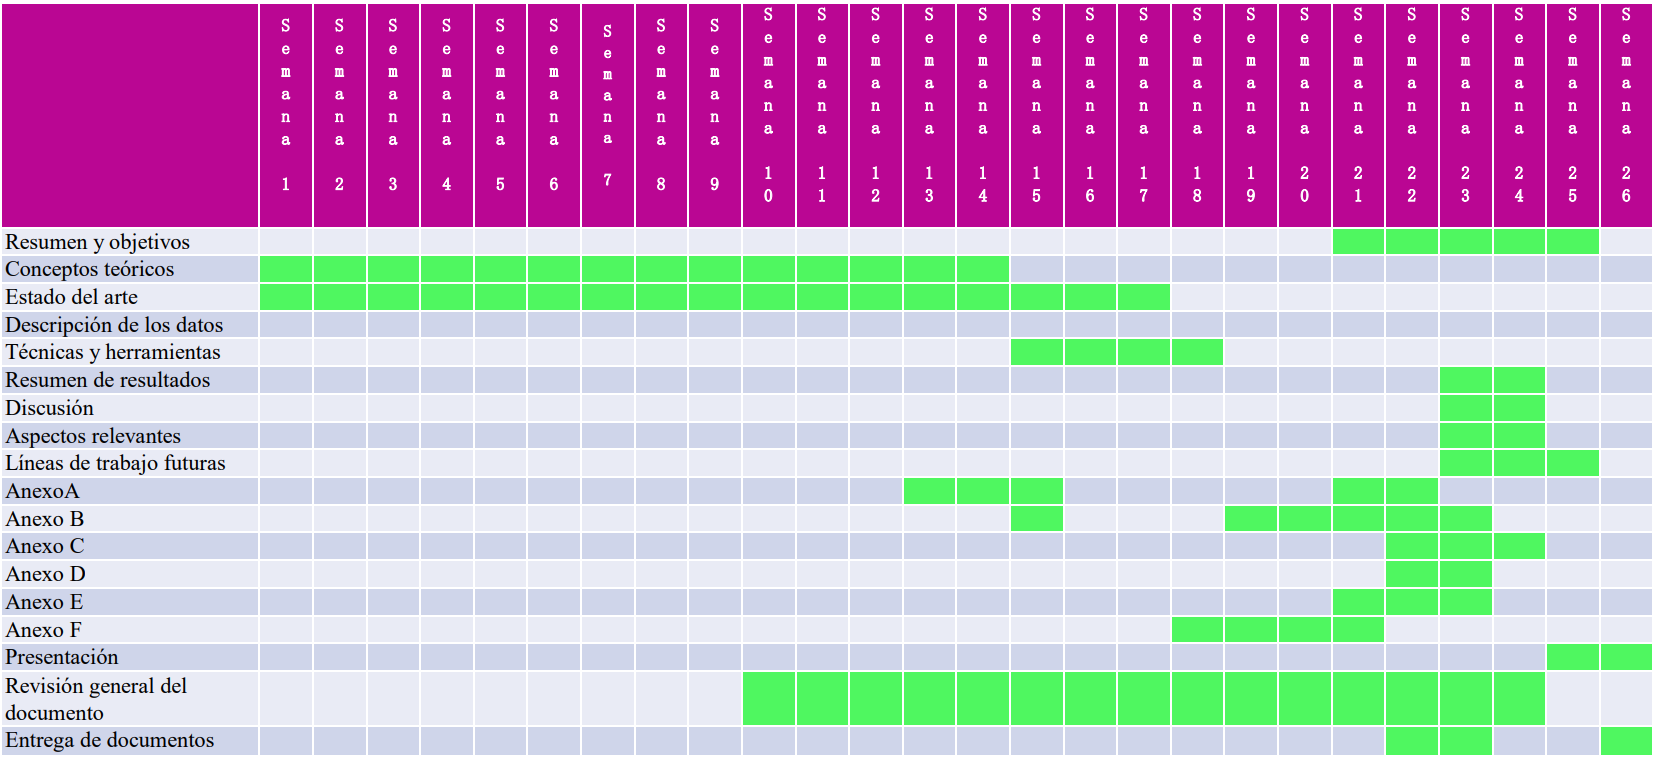
\includegraphics[width=1\textwidth]{img/PlanificacionTemporal.png}
    \caption{Planificación temporal seguida para la realización de este proyecto.  Fuente propia.}
    \label{fig:planTemporal} 
\end{figure}

En la planificación temporal se puede ver cada apartado de la memoria y los anexos desarrollados a lo largo de las semanas. 

\section{Planificación económica}

Para obtener una buena planificación económica se deberán identificar los costes tanto personales como materiales y de desarrollo y los ingresos relacionados con el prototipo.

Los costes personales se calcularán en función del salario medio de un Ingeniero de la Salud durante un periodo aproximado de 6 meses durante media jornada\footnote{La media jornada constará de unas 4 horas al día durante 5 días a la semana, es decir, 20 horas semanales.}, lo que suma unas 540 horas de trabajo totales. Teniendo en cuenta que el sueldo neto medio de un ingeniero con menos de 3 años de experiencia ronda los 1392,8€ al mes a jornada completa \cite{SueldoBruto}, a media jornada cobrará unos 696,4€ al mes. Por lo tanto, los costes de personal se podrían resumir en la siguiente tabla.

% ----------------------------------------------------
% Tabla del desglose económico de costes personales.
\begin{table}[h!]
\centering
\begin{tabular}{ |m{5cm} m{3cm}|  } 
\hline
\cellcolor[HTML]{EFEFEF}\textbf{} & \cellcolor[HTML]{EFEFEF}\textbf{Costes}\\

Sueldo neto mensual           & {696,4€} \\

Sueldo bruto mensual                & {799,79€}\\
\hline
\cellcolor[HTML]{EFEFEF}\textbf{Total en los 6 meses}                & \cellcolor[HTML]{EFEFEF}{4798,74€} \\
\hline
\end{tabular}
\caption{Resumen de costes personales.}
\end{table}

Como primeros gastos relacionados con los equipos de desarrollo, el ordenador que se ha empleado y la licencia de Office que se ha empleado para la realización de algunas partes del proyecto, con una amortización\footnote{La amortización se calcula con la diferencia del coste del equipo y del coste residual a los 4 años (un 40\% del coste del equipo) todo ello divido entre el periodo de amortización, que en este caso serán unos 4 años.} \cite{amortizacion} en unos 4 años. No se incluyen gastos de otros softwares, porque se han empleado herramientas de código abierto y gratuitas.

% ----------------------------------------------------
% Tabla del desglose económico de equipos de desarrollo.
\begin{table}[h!]
\centering
\begin{tabular}{ |m{5cm} m{3cm} m{3cm}|  } 
\hline
\cellcolor[HTML]{EFEFEF}\textbf{} & \cellcolor[HTML]{EFEFEF}\textbf{Costes}& \cellcolor[HTML]{EFEFEF}\textbf{Amortización}\\

Ordenador ASUS           & {700€} & {105€}\\

Office 365 personal anual              & {69€} & {10,35€}\\
\hline
\cellcolor[HTML]{EFEFEF}\textbf{Total en los 6 meses}                & \cellcolor[HTML]{EFEFEF}{769€} & \cellcolor[HTML]{EFEFEF}{115,35€} \\
\hline
\end{tabular}
\caption{Resumen de costes de equipos de desarrollo amortizados en 4 años.}
\end{table}


Para el cálculo del gasto de los materiales del desarrollo del prototipo, se tienen en cuenta los costes de los componentes y los gastos de realización del prototipo, mientras que para obtener los posibles ingresos se tendrá en cuenta el beneficio, gastos imprevistos e I+D del producto, para posibles mejoras en e futuro. La suma de gastos e ingresos nos devolverá el precio final aproximado del dispositivo. No se incluyen los gastos personales, ni de equipos, dado que estos gastos se incluirían en caso de producción del dispositivo final.


% ----------------------------------------------------
% Tabla del desglose económico de las versiones realizadas.
\begin{table}[h!]
\centering
\begin{tabular}{ |m{4cm}|m{4cm}|m{2cm}|m{2cm}|  } 
\hline
\cellcolor[HTML]{B9E3F0}\textbf{} & \cellcolor[HTML]{B9E3F0}\textbf{Cálculos} & \cellcolor[HTML]{B9E3F0}\textbf{Versión 1}& \cellcolor[HTML]{B9E3F0}\textbf{Versión 2}\\

\hline
\cellcolor[HTML]{EFEFEF}\textbf{Gastos de los componentes}             & {Suma de los precios de cada componente del producto}   & 27€ & 32.5€\\
\hline
\cellcolor[HTML]{EFEFEF}\textbf{Gastos de producción}                & {10\% del precio de los componentes} & 2.7€ & 3.25€\\
\hline
\cellcolor[HTML]{EFEFEF}\textbf{Ingresos destinados a beneficio}                & {5\% del total de gastos} & 1.48€ & 1.79€\\
\hline
\cellcolor[HTML]{EFEFEF}\textbf{Gastos imprevistos e I+D} & {10\% del total de gastos} & 2.97€ & 3.58€\\
\hline
\cellcolor[HTML]{EFEFEF}\textbf{Precio Total} & {Suma de los gastos e ingresos} & \textbf{34.15€} & \textbf{41.10€}\\
\hline
\end{tabular}
\caption{Resumen de gastos y precio total del producto}
\end{table}

El prototipo de la versión 1, en la que se emplea el sensor SW520D\cite{SW520D_1}, tiene un coste final aproximado\footnote{La planificación económica será variable en el tiempo y durante el desarrollo del producto, por lo que se trata de precios totales aproximados. Igual para el prototipo versión 2.} de unos 34.15€, precio que podría ser menor al crear nuestro propio microcontrolador o utilizar una alternativa similar a Arduino, puesto que es el elemento que más aumenta el precio de la solución, siendo el precio del resto de los componentes aproximadamente unos 3€.

Por el contrario el prototipo de la versión 2, en el que se emplea el módulo MPU-6050\cite{MPU6050_1,MPU6050_2}, tiene un coste final aproximado de unos 41.10€, precio que también podría disminuir al crear nuestro propio microcontrolador o utilizar una alternativa a Arduino, ya que sin el microcontrolador Arduino el precio ronda los 8.5€.


\subsection{Desglose de los precios de los componentes del prototipo Versión 1}

Se han tenido en cuenta los precios más bajos encontrados de cada componente necesario. Estos precios incluyen el porcentaje de IVA y se han calculado en base a los precios del proveedor Amazon España\cite{amazon}.
\begin{itemize}
    \item Arduino UNO R3: 24€
    \item Resistencias (330 \textOmega, 2x220 \textOmega, 33 \textOmega, 1000 \textOmega): 0.05€
    \item Zumbador pasivo: 0.25€
    \item Motor de vibración: 1€
    \item Transistor: 0.05€
    \item SW520D: 0.5€
    \item Led azul: 0.02€
    \item Pulsador: 0.05€
    \item Otros elementos variados: 1€
    
\end{itemize}

\subsection{Desglose de los precios de los componentes del prototipo Versión 2}
Se han tenido en cuenta los precios más bajos encontrados de cada componente necesario. Estos precios incluyen el porcentaje de IVA y se han calculado en base a los precios del proveedor Amazon España\cite{amazon}.
\begin{itemize}
    \item Arduino UNO R3: 24€
    \item Resistencias (2x330 \textOmega, 2x220 \textOmega, 33 \textOmega, 1000 \textOmega): 0.06€
    \item Zumbador pasivo: 0.25€
    \item Motor de vibración: 1€
    \item Transistor NPN: 0.05€
    \item MPU-6050: 6€
    \item Led azul: 0.02€
    \item 2x Pulsador: 0.10€
    \item Otros elementos variados: 1€
    
\end{itemize}


\section{Viabilidad legal}

Se debe tener en cuenta en todo momento que el dispositivo sea completamente seguro y no afecte negativamente al usuario. Para ello, existen legislaciones específicas a cada fase del desarrollo y comercialización del producto que se deben cumplir para obtener un dispositivo seguro y regulado.

Se pueden diferenciar 3 fases, una primera fase de creación de la idea, diseño y desarrollo y realización de pruebas, una segunda fase de comercialización y la última fase de posventa, donde se incluyen las demandas y la gestión de los datos de los usuarios.

Durante la primera fase de creación de la idea, diseño y desarrollo del producto y realización de pruebas, todos los movimientos que se realicen se deberán ajustar a las siguientes legislaciones:
\begin{itemize}
    \item Ley 24/2015\cite{patentes}, Ley de Patentes, dónde se regula todo lo relacionado con la protección de invenciones empleando patentes, desde el registro de las patentes, invenciones patentables, el derecho a la patente y los procedimientos para pedir una patente.
    % Referencia: 
    % https://www.boe.es/buscar/act.php?id=BOE-A-2015-8328
    
    \item Real Decreto Legislativo 1/1996\cite{PropIntelectual} relativo Ley de Propiedad Intelectual que regulariza la protección del derecho de autor y de derechos similares.
    % referencia:
    % https://boe.es/buscar/act.php?id=BOE-A-1996-8930
    
    \item Los productos sanitarios se rigen por la Agencia española de medicamentos y productos sanitarios (AEMPS)\cite{AEMPS}. En este proyecto nos interesan especialmente el Real Decreto 1591/2009\cite{prodSanitario1} que regula todo lo relativo a los productos sanitarios, desde su desarrollo a su venta, y el Real Decreto 437/2002\cite{prodSanitario2} establece las pautas para la concesión de licencias de fabricación y desarrollo de productos sanitarios.
    % Referencias:
    % https://www.aemps.gob.es/productos-sanitarios/legislacion-sobre-productos-sanitarios/
    % https://www.boe.es/buscar/doc.php?id=BOE-A-2009-17606
    % https://www.boe.es/buscar/doc.php?id=BOE-A-2002-10228
    
    \item Reglamento de la UE 2017/745\cite{ProdSanitariosEU} de Productos Sanitarios de la Unión Europea este reglamento establece requisitos y regula la comercialización de productos sanitarios en la Unión Europea, con el fin de garantizar un dispositivo de calidad, eficaz y completamente seguro.
    % Referencia:
    % https://eur-lex.europa.eu/legal-content/ES/TXT/?uri=uriserv:OJ.L_.2017.117.01.0001.01.SPA&toc=OJ:L:2017:117:TOC
    
    \item Además, durante todo el desarrollo del producto se deberá cumplir con la normativa laboral española\cite{normaLaboral}, que incluye leyes y reglamentos como pueden ser el Estatuto de los Trabajadores, la Ley de Prevención de Riesgos Laborales o la Ley de Igualdad.
    % Referencia
    % https://www.boe.es/biblioteca_juridica/codigos/codigo.php?id=93&modo=2&nota=0&tab=2
    
\end{itemize}

Si se consigue crear el dispositivo en base a todas las leyes anteriores y se quisiera sacar a mercado se deberán cumplir también con los siguientes requisitos legales:
\begin{itemize}
    \item La Ley 34/2002\cite{comercioElectronico} de Servicios de la Sociedad de la Información y de Comercio Electrónico, en caso de que se realice una tienda web oficial de comercialización del dispositivo.
    % Referencia:
    % https://www.boe.es/buscar/act.php?id=BOE-A-2002-13758
    
    \item Además, se deberán tener en cuenta otras leyes\cite{comercio} como la Ley 7/1996\cite{comercioMinorista} de Ordenación del Comercio Minorista.
    % Referencia:
    % https://www.boe.es/buscar/act.php?id=BOE-A-1996-1072
    % https://www.boe.es/biblioteca_juridica/codigos/codigo.php?id=35&modo=2&nota=0&tab=2
\end{itemize}

Por último, si el dispositivo se ha puesto a la venta se debe pensar en los requisitos legales que se necesitarán cumplir a partir del momento de la primera venta. Alguno de estos requisitos serán:
\begin{itemize}
    \item Ley Orgánica 3/2018\cite{protDatos} de Protección de Datos Personales y garantía de los derechos digitales. Para poder proteger cualquier información que identifique a una persona, de forma confidencial. Además, el usuario debe estar correctamente informado del tratamiento de sus datos, además el acceso al tratamiento de sus datos debe ser claro y accesible.

    El usuario tendrá derecho al acceso de sus datos, derecho de rectificación y supresión de sus datos, derecho a la limitación del tratamiento de sus datos, derecho a la portabilidad de sus datos y el derecho a oponerse al tratamiento de sus datos. Por todo ello el tratamiento de sus datos debe ser tras la confirmación clara del consentimiento informado del tratamiento de sus datos.
    % Referencia:
    % https://www.boe.es/buscar/doc.php?id=BOE-A-2018-16673

    \item Reglamento UE 2016/679\cite{protDatosEU} relativo a Protección de las Personas Físicas en lo que respecta al tratamiento de datos personales y circulación de estos Datos. Donde se define que se debe garantizar la protección de los datos con los que se trabaja, además de notificar brechas de seguridad o exposición de datos al usuario.
    % Referencia:
    % https://eur-lex.europa.eu/ES/legal-content/summary/general-data-protection-regulation-gdpr.html
\end{itemize}

Además el dispositivo deberá contar con un certificado CE\cite{certificadoEuropeo}, que garantizará que el dispositivo cumple con los requisitos de seguridad, protección y sanidad europeos. Una vez se obtenga el certificado el dispositivo podrá ser comercializado legalmente en la Unión Europea.
% Referencia:
% https://europa.eu/youreurope/business/product-requirements/labels-markings/ce-marking/index_es.htm
\apendice{Documentación de usuario}

\section{Requisitos software y hardware para ejecutar el proyecto.}

\section{Instalación / Puesta en marcha}

\section{Manuales y/o Demostraciones prácticas}




    
     
\apendice{Manual del desarrollador / programador / investigador.} % usar el término que mejor se corresponda.

\section{Estructura de directorios}

Descripción de los directorios y ficheros entregados. (De github, entiendo, o también la propia aplicación si se llega a obtener)

\section{Compilación, instalación y ejecución del proyecto}

En caso de ser necesaria esta sección, porque la compilación o ejecución no sea directa.


\section{Pruebas del sistema}
Esta sección puede ser opcional.

Puede tratarse de validación de la interfaz por parte de los usuarios, mediante escuestas o similar o validación del funcionamiento mediante pruebas unitarias.



\section{Instrucciones para la modificación o mejora del proyecto.}

Instrucciones y consejos para que el trabajo pueda ser mejorado en futuras ediciones.
\apendice{Descripción de adquisición y tratamiento de datos}

Va fuera creo simplemente con la información del punto de descripcion de los datos de la memoria será suficiente.

\textcolor{red}{cuando hables de los datos, como los habrás generado y recogido tu habla de ELABORACiÖN PROPIA.}

\section{Descripción formal de los datos}

Tablas, imágenes, señales, secuencias de ADN…
    
\section{Descripción clínica de los datos.}

Descripción y explicaciones clinicas del significado o interpretación de los datos.
\apendice{Manual de especificación de diseño}
En este anexo se propone la realización de los diagramas de despliegue correspondientes al desarrollo del proyecto.

No se ha realizado ningún diagrama de despliegue específico para ninguna de las versiones propuestas puesto que no se ha llegado a crear la aplicación móvil de interacción de usuario-prototipo y tampoco se han definido clases en los programas de Arduino\cite{ArduinoIDE} creados para cada una de las versiones. 

Sin embargo, se ha creado un diagrama común para la visualización de las funciones, atributos y nodos correspondientes a los prototipos. Se pueden ver las distintas funciones y atributos en el diagrama \ref{fig:digDespliegue}:

% Inicio de la figura
\begin{figure}[h]
    \centering
    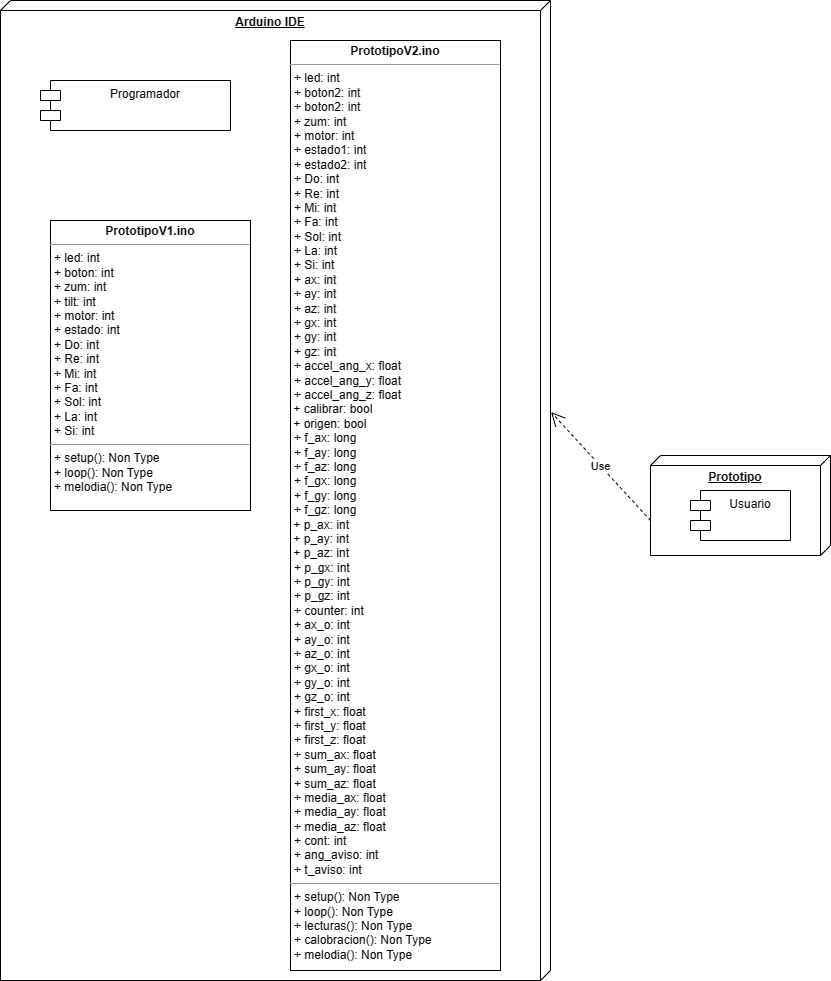
\includegraphics[width=0.8\textwidth]{img/DiagramDespliegue.png}
    \caption{Diagrama de los programas de los prototipos. Fuente propia.}
    \label{fig:digDespliegue} 
\end{figure}



\apendice{Especificación de Requisitos}

Si procede.


\section{Diagrama de casos de uso}

% Inicio de la figura
\begin{figure}[h]
    \centering
    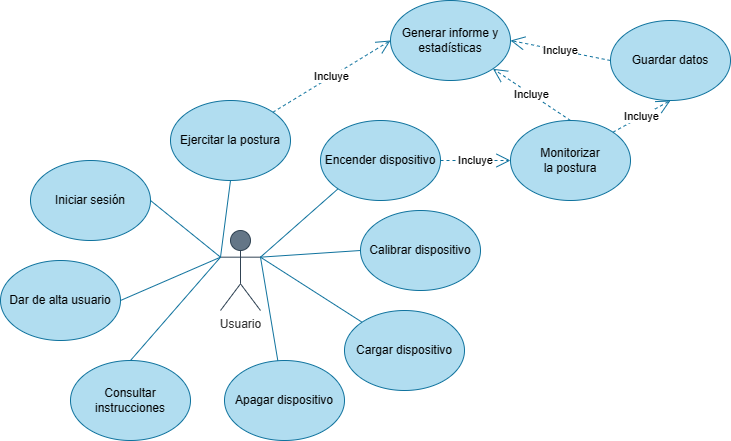
\includegraphics[width=1\textwidth]{img/DiagramaCasosDeUso.png}
    \caption{Diagrama de casos de uso}
    \label{fig:Casosuso} % Esta etiqueta es la que permite que se encuentr referenciada en el texto (es muy importante que siempre estén referenciadas en el texto)
\end{figure}

\section{Explicación casos de uso.}



Se puede describir mediante el uso de tablas o mediante lenguaje natural.   

Una muestra de cómo podría ser una tabla de casos de uso:

\begin{comment}
% Caso de Uso 1 -> Consultar Experimentos.
\begin{table}[p]
	\centering
	\begin{tabularx}{\linewidth}{ p{0.21\columnwidth} p{0.71\columnwidth} }
		%\toprule
		\multicolumn{1}{|l|} {\cellcolor[HTML]{68CBD0}\textbf{CU-1}}    & \multicolumn{1}{l|}{\textbf{Ejemplo de caso de uso}}\\
		%\toprule
		\textbf{Versión}              & 1.0    \\
		\textbf{Autor}                & Alumno \\
		\textbf{Requisitos asociados} & RF-xx, RF-xx \\
		\textbf{Descripción}          & La descripción del CU \\
		\textbf{Precondición}         & Precondiciones (podría haber más de una) \\
		\textbf{Acciones}             &
		\begin{enumerate}
			\def\labelenumi{\arabic{enumi}.}
			\tightlist
			\item Pasos del CU
			\item Pasos del CU (añadir tantos como sean necesarios)
		\end{enumerate}\\
		\textbf{Postcondición}        & Postcondiciones (podría haber más de una) \\
		\textbf{Excepciones}          & Excepciones \\
		\textbf{Importancia}          & Alta o Media o Baja... \\
		\bottomrule
	\end{tabularx}
	\caption{CU-1 Nombre del caso de uso.}
\end{table}
\end{comment}


% Comentamos las tablas de ejemplo
\begin{comment}
% Caso de Uso 2 -> Consultar Experimentos.
\begin{table}[p]
	\centering
        
	\begin{tabularx}{\linewidth}{ p{0.21\columnwidth} p{0.71\columnwidth} }
		%\toprule
        \hline
		\multicolumn{3}{|c|} {\cellcolor[HTML]{68CBD0}\textbf{CU-1}}    & \multicolumn{1}{|c|}{\textbf{Ejemplo de caso de uso}}\\
		%\toprule
  \hline
		\multicolumn{1}{|l|}{\textbf{Versión}}              & 1.0    \\
		\textbf{Autor}                & Alumno \\
		\textbf{Requisitos asociados} & RF-xx, RF-xx \\
		\textbf{Descripción}          & La descripción del CU \\
		\textbf{Precondición}         & Precondiciones (podría haber más de una) \\
		\textbf{Acciones}             &
		\begin{enumerate}
			\def\labelenumi{\arabic{enumi}.}
			\tightlist
			\item Pasos del CU
			\item Pasos del CU (añadir tantos como sean necesarios)
		\end{enumerate}\\
		\textbf{Postcondición}        & Postcondiciones (podría haber más de una) \\
		\textbf{Excepciones}          & Excepciones \\
		\textbf{Importancia}          & Alta o Media o Baja... \\
		\bottomrule
	\end{tabularx}
	\caption{CU-2 Nombre del caso de uso.}
\end{table}
\end{comment}

% ----------------------------------------------------
% ----------------------------------------------------
% Caso de uso 01
\begin{table}[h!]
\centering
\begin{tabular}{ |m{3cm}|m{11cm}|  } 
\hline
\cellcolor[HTML]{B9E3F0}\centering\textbf{CS-01} & \cellcolor[HTML]{B9E3F0}\textbf{<Encender dispositivo>}\\

\hline
\cellcolor[HTML]{EFEFEF}\textbf{Versión}             & 1.0  \\
\hline
\cellcolor[HTML]{EFEFEF}\textbf{Autor}                & Naiara Gadea Rodíguez Gómez\\
\hline
\cellcolor[HTML]{EFEFEF}\textbf{Descripción}                & {Puesta en marcha del dispositivo hardware y su conexión con la aplicación. El dispositivo no deberá estar siempre conectado con la aplicación, pero si se conecta a la aplicación se puede obtener más información. }\\
\hline
\cellcolor[HTML]{EFEFEF}\textbf{Secuencia \newline Normal}                &                 
        \begin{enumerate}
			\def\labelenumi{\arabic{enumi}.}
			\tightlist
			\item Se coloca el dispositivo en contacto sobre la piel, como se indica en las instrucciones.
			\item Se enciende el dispositivo con el botón ON/OFF.
                \item Cuando se encienda un led verde indicará que el dispositivo está encendido.  
                \item Se conecta el dispositivo al dispositivo que tiene instalada la aplicación vía Bluetooth o vía WIFI.
                \item El usuario accede a la aplicación software instalada en el dispositivo móvil o en el ordenador, que deberán estar conectados a la misma red WIFI o Bluetooth para permitir la comunicación.  
                \item Una vez se realiza la conexión, el led verde del dispositivo cambia a color a azul. Además, en la aplicación aparece el dispositivo como conectado. 
		\end{enumerate}\\
\hline
\cellcolor[HTML]{EFEFEF}\textbf{Frecuencia}                & Alta\\
\hline
\cellcolor[HTML]{EFEFEF}\textbf{Importancia}                & Alta\\
\hline
\cellcolor[HTML]{EFEFEF}\textbf{Urgencia}                & Alta\\
\hline
\cellcolor[HTML]{EFEFEF}\textbf{Requisitos Funcionales Relacionados}                & {RF-02}\\
\hline
\cellcolor[HTML]{EFEFEF}\textbf{Casos de uso relacionados}                & {CS-02, CS-03, CS-04, CS-07, CS-08, CS-10}\\
\hline
\end{tabular}
\caption{CU-01. Encender dispositivo.}
\end{table}

% ----------------------------------------------------
% Caso de uso 02
\begin{table}[h!]
\centering
\begin{tabular}{ |m{3cm}|m{11cm}|  } 
\hline
\cellcolor[HTML]{B9E3F0}\textbf{CS-02} & \cellcolor[HTML]{B9E3F0}\textbf{<Apagar dispositivo>}\\

\hline
\cellcolor[HTML]{EFEFEF}\textbf{Versión}             & 1.0  \\
\hline
\cellcolor[HTML]{EFEFEF}\textbf{Autor}                & Naiara Gadea Rodíguez Gómez\\
\hline
\cellcolor[HTML]{EFEFEF}\textbf{Descripción}                & {Apagado del dispositivo.}\\
\hline
\cellcolor[HTML]{EFEFEF}\textbf{Secuencia \newline Normal}                &                 
        \begin{enumerate}
			\def\labelenumi{\arabic{enumi}.}
			\tightlist
			\item Se apaga el dispositivo con el botón ON/OFF.
			\item Una vez el dispositivo se encuentre apagado el led azul o verde se apagará.
                \item El usuario se puede quitar el dispositivo y puede cargarlo.
		\end{enumerate}\\
\hline
\cellcolor[HTML]{EFEFEF}\textbf{Frecuencia}                & Alta\\
\hline
\cellcolor[HTML]{EFEFEF}\textbf{Importancia}                & Alta\\
\hline
\cellcolor[HTML]{EFEFEF}\textbf{Urgencia}                & Media\\
\hline
\cellcolor[HTML]{EFEFEF}\textbf{Requisitos Funcionales Relacionados}                & {RF-02}\\
\hline
\cellcolor[HTML]{EFEFEF}\textbf{Casos de uso relacionados}                & {CS-01, CS-03}\\
\hline
\cellcolor[HTML]{EFEFEF}\textbf{Comentarios}                & {El dispositivo también se apaga cuando se acaba la batería, en cuyo caso el caso de uso comienza en el paso 2. }\\
\hline
\end{tabular}
\caption{CU-02. Apagar dispositivo.}
\end{table}

% ----------------------------------------------------
% Caso de uso 03
\begin{table}[h!]%[p]
\centering
\begin{tabular}{ |m{3cm}|m{11cm}|  } 
\hline
\cellcolor[HTML]{B9E3F0}\textbf{CS-03} & \cellcolor[HTML]{B9E3F0}\textbf{<Cargar dispositivo>}\\

\hline
\cellcolor[HTML]{EFEFEF}\textbf{Versión}             & 1.0  \\
\hline
\cellcolor[HTML]{EFEFEF}\textbf{Autor}                & Naiara Gadea Rodíguez Gómez\\
\hline
\cellcolor[HTML]{EFEFEF}\textbf{Descripción}                & {Carga de la batería del dispositivo empleando la estación de carga.}\\
\hline
\cellcolor[HTML]{EFEFEF}\textbf{Secuencia \newline Normal}                &                 
        \begin{enumerate}
			\def\labelenumi{\arabic{enumi}.}
			\tightlist
			\item Actúa el CS-02. 
			\item Una vez que el dispositivo se encuentre apagado el usuario coloca el dispositivo sobre la estación de carga enchufada a la corriente.
                \item Se enciende un led rojo intermitente.
                \item Cuando la batería del dispositivo se encuentre completamente cargada, el led rojo intermitente deja de ser intermitente.
                \item El dispositivo está completamente cargado y puede desconectar la estación de carga de la corriente o desconectar el dispositivo.
                \item El dispositivo estará listo para su uso.
		\end{enumerate}\\
\hline
\cellcolor[HTML]{EFEFEF}\textbf{Frecuencia}                & Alta\\
\hline
\cellcolor[HTML]{EFEFEF}\textbf{Importancia}                & Alta\\
\hline
\cellcolor[HTML]{EFEFEF}\textbf{Urgencia}                & Media\\
\hline
\cellcolor[HTML]{EFEFEF}\textbf{Requisitos Funcionales Relacionados}                & {RF-08}\\
\hline
\cellcolor[HTML]{EFEFEF}\textbf{Casos de uso relacionados}                & {CS-02}\\
\hline
\end{tabular}
\caption{CU-03. Cargar dispositivo.}
\end{table}

% ----------------------------------------------------
% Caso de uso 04
\begin{table}[h!]
\centering
\begin{tabular}{ |m{3cm}|m{11cm}|  } 
\hline
\cellcolor[HTML]{B9E3F0}\textbf{CS-04} & \cellcolor[HTML]{B9E3F0}\textbf{<Calibrar dispositivo>}\\

\hline
\cellcolor[HTML]{EFEFEF}\textbf{Versión}             & 1.0  \\
\hline
\cellcolor[HTML]{EFEFEF}\textbf{Autor}                & Naiara Gadea Rodíguez Gómez\\
\hline
\cellcolor[HTML]{EFEFEF}\textbf{Descripción}                & {Se recalculan los valores en reposo para que el dispositivo devuelva medidas lo más precisas posible. Se debe calibrar el dispositivo cada cierto tiempo para que los valores medidos sean lo más precisos posible.}\\
\hline
\cellcolor[HTML]{EFEFEF}\textbf{Secuencia \newline Normal}                &                 
        \begin{enumerate}
			\def\labelenumi{\arabic{enumi}.}
			\tightlist
			\item El dispositivo debe estar encendido y sobre una superficie plana.
			\item Se presionará el botón de calibrado. Sobre el dispositivo o de la propia aplicación. 
                \item El sistema recalibra los valores medidos por el dispositivo.
                \item Una vez el dispositivo se haya calibrado correctamente se encenderá 3 veces el led verde o azul, en función si la calibración se ha realizado a través de la aplicación o directamente sobre el dispositivo. 
                \item El dispositivo se encuentra correctamente calibrado y listo para su uso. 
		\end{enumerate}\\
\hline
\cellcolor[HTML]{EFEFEF}\textbf{Frecuencia}                & Baja\\
\hline
\cellcolor[HTML]{EFEFEF}\textbf{Importancia}                & Alta\\
\hline
\cellcolor[HTML]{EFEFEF}\textbf{Urgencia}                & Baja\\
\hline
\cellcolor[HTML]{EFEFEF}\textbf{Requisitos Funcionales Relacionados}                & {RF-01, RF-04}\\
\hline
\cellcolor[HTML]{EFEFEF}\textbf{Casos de uso relacionados}                & {CS-01, CS-07}\\
\hline
\end{tabular}
\caption{CU-04. Calibrar dispositivo.}
\end{table}

% ----------------------------------------------------
% Caso de uso 05
\begin{table}[h!]
\centering
\begin{tabular}{ |m{3cm}|m{11cm}|  } 
\hline
\cellcolor[HTML]{B9E3F0}\textbf{CS-05} & \cellcolor[HTML]{B9E3F0}\textbf{<Dar de alta usuario>}\\

\hline
\cellcolor[HTML]{EFEFEF}\textbf{Versión}             & 1.0  \\
\hline
\cellcolor[HTML]{EFEFEF}\textbf{Autor}                & Naiara Gadea Rodíguez Gómez\\
\hline
\cellcolor[HTML]{EFEFEF}\textbf{Descripción}                & {El usuario crea una cuenta para cada recopilar los datos recopilados por el dispositivo. Se creará una cuenta por persona que vaya a utilizar el dispositivo.}\\
\hline
\cellcolor[HTML]{EFEFEF}\textbf{Secuencia \newline Normal}                &                 
        \begin{enumerate}
			\def\labelenumi{\arabic{enumi}.}
			\tightlist
			\item El caso de uso comienza cuando el facultativo clica en registrar.
			\item El sistema solicita el nombre de usuario. 
                \item El usuario introduce el nombre de usuario.
                \item El sistema solicita los nombre y apellidos del usuario.
                \item El usuario introduce su nombre y apellidos.
                \item El sistema solicita una contraseña. 
                \item El usuario introduce una contraseña. 
                \item El sistema guarda y almacena los datos introducidos. Se ha creado la cuenta del usuario. 
		\end{enumerate}\\
\hline
\cellcolor[HTML]{EFEFEF}\textbf{Frecuencia}                & Baja\\
\hline
\cellcolor[HTML]{EFEFEF}\textbf{Importancia}                & Media\\
\hline
\cellcolor[HTML]{EFEFEF}\textbf{Urgencia}                & Media\\
\hline
\cellcolor[HTML]{EFEFEF}\textbf{Requisitos Funcionales Relacionados}                & {RF-01, RF-03 }\\
\hline
\cellcolor[HTML]{EFEFEF}\textbf{Casos de uso relacionados}                & {CS-06}\\
\hline
\end{tabular}
\caption{CU-05. Dar de alta usuario.}
\end{table}

% ----------------------------------------------------
% Caso de uso 06
\begin{table}[h!]
\centering
\begin{tabular}{ |m{3cm}|m{11cm}|  } 
\hline
\cellcolor[HTML]{B9E3F0}\textbf{CS-06} & \cellcolor[HTML]{B9E3F0}\textbf{<Iniciar sesión>}\\

\hline
\cellcolor[HTML]{EFEFEF}\textbf{Versión}             & 1.0  \\
\hline
\cellcolor[HTML]{EFEFEF}\textbf{Autor}                & Naiara Gadea Rodíguez Gómez\\
\hline
\cellcolor[HTML]{EFEFEF}\textbf{Descripción}                & {El usuario inicia sesión en la aplicación para poder acceder a sus datos, informes y ejercicios. El usuario tiene la opción de mantener la sesión iniciada. }\\
\hline
\cellcolor[HTML]{EFEFEF}\textbf{Secuencia \newline Normal}                &                 
        \begin{enumerate}
			\def\labelenumi{\arabic{enumi}.}
			\tightlist
			\item El sistema solicita nombre de usuario y contraseña.
			\item El usuario introduce su nombre de usuario y contraseña. 
                \item El sistema pregunta si desea mantener la sesión abierta.
                \item El usuario introduce si desea mantener la sesión abierta. 
                \item El sistema compara con su base de datos y si encuentra coincidencia accede a los datos del usuario. En caso de que no encuentre al usuario el sistema imprime por pantalla ‘Contraseña o usuario incorrectos’.
                \item El sistema muestra las estadísticas y datos del paciente.
		\end{enumerate}\\
\hline
\cellcolor[HTML]{EFEFEF}\textbf{Frecuencia}                & Media\\
\hline
\cellcolor[HTML]{EFEFEF}\textbf{Importancia}                & Alta\\
\hline
\cellcolor[HTML]{EFEFEF}\textbf{Urgencia}                & Media\\
\hline
\cellcolor[HTML]{EFEFEF}\textbf{Requisitos Funcionales Relacionados}                & {RF-01, RF-03, RF-06 }\\
\hline
\cellcolor[HTML]{EFEFEF}\textbf{Casos de uso relacionados}                & {CS-05, CS-07, CS-08, CS-09, CS-10}\\
\hline
\cellcolor[HTML]{EFEFEF}\textbf{Comentarios}                & {Si el usuario ha indicado que desea mantener la sesión abierta, la sesión se mantiene abierta, aunque se cierre la aplicación. El usuario deberá cerrar manualmente su sesión. }\\
\hline
\end{tabular}
\caption{CU-06. Iniciar sesión.}
\end{table}

% ----------------------------------------------------
% Caso de uso 07
\begin{table}[h!]
\centering
\begin{tabular}{ |m{3cm}|m{11cm}|  } 
\hline
\cellcolor[HTML]{B9E3F0}\textbf{CS-07} & \cellcolor[HTML]{B9E3F0}\textbf{<Realizar monitoreo de la postura>}\\

\hline
\cellcolor[HTML]{EFEFEF}\textbf{Versión}             & 1.0  \\
\hline
\cellcolor[HTML]{EFEFEF}\textbf{Autor}                & Naiara Gadea Rodíguez Gómez\\
\hline
\cellcolor[HTML]{EFEFEF}\textbf{Descripción}                & {Una vez el dispositivo se encuentre encendido se realiza la monitorización de la postura. Si se detecta una mala postura el dispositivo emitirá una vibración. En el caso de que el dispositivo se encuentre conectado con la aplicación los datos.}\\
\hline
\cellcolor[HTML]{EFEFEF}\textbf{Secuencia \newline Normal}                &                 
        \begin{enumerate}
			\def\labelenumi{\arabic{enumi}.}
			\tightlist
			\item El caso de uso comienza cuando se enciende el usuario enciende el dispositivo. 
			\item Pasos del CU El sistema obtiene los datos proporcionados por el sensor del dispositivo. 
                \item El sistema identifica entre una buena o mala postura, gracias al algoritmo. 
                \item Si se detecta mala postura el dispositivo emita una señal vibratoria para que el usuario modifique su postura.
                \item Interviene el CS-08. 
                \item El caso de uso finaliza cuando se apaga el dispositivo o cuando se gasta la batería del dispositivo.
		\end{enumerate}\\
\hline
\cellcolor[HTML]{EFEFEF}\textbf{Frecuencia}                & Alta\\
\hline
\cellcolor[HTML]{EFEFEF}\textbf{Importancia}                & Alta\\
\hline
\cellcolor[HTML]{EFEFEF}\textbf{Urgencia}                & Alta\\
\hline
\cellcolor[HTML]{EFEFEF}\textbf{Requisitos Funcionales Relacionados}                & {RF-02, RF-04, RF-05 }\\
\hline
\cellcolor[HTML]{EFEFEF}\textbf{Casos de uso relacionados}                & {CS- 01, CS-04, CS-06, CS-08, CS-09, CS-10 }\\
\hline
\end{tabular}
\caption{CU-07. Realizar monitoreo de la postura.}
\end{table}

% ----------------------------------------------------
% Caso de uso 08
\begin{table}[h!]
\centering
\begin{tabular}{ |m{3cm}|m{11cm}|  } 
\hline
\cellcolor[HTML]{B9E3F0}\textbf{CS-08} & \cellcolor[HTML]{B9E3F0}\textbf{<Guardar datos>}\\

\hline
\cellcolor[HTML]{EFEFEF}\textbf{Versión}             & 1.0  \\
\hline
\cellcolor[HTML]{EFEFEF}\textbf{Autor}                & Naiara Gadea Rodíguez Gómez\\
\hline
\cellcolor[HTML]{EFEFEF}\textbf{Descripción}                & {Se archivan los datos recopilados a través del dispositivo. Los datos se van guardando en tiempo real si el dispositivo se encuentra conectado a la aplicación.}\\
\hline
\cellcolor[HTML]{EFEFEF}\textbf{Secuencia \newline Normal}                &                 
        \begin{enumerate}
			\def\labelenumi{\arabic{enumi}.}
			\tightlist
			\item El sistema registra los datos enviados vía Bluetooth o WIFI por el dispositivo.
			\item Interviene el CS-07.
                \item El sistema guarda los datos y el informe generado en la base de datos integrada. Que se podrán consultar posteriormente o en tiempo real.
		\end{enumerate}\\
\hline
\cellcolor[HTML]{EFEFEF}\textbf{Frecuencia}                & Alta\\
\hline
\cellcolor[HTML]{EFEFEF}\textbf{Importancia}                & Alta\\
\hline
\cellcolor[HTML]{EFEFEF}\textbf{Urgencia}                & Alta\\
\hline
\cellcolor[HTML]{EFEFEF}\textbf{Requisitos Funcionales Relacionados}                & {RF-01, RF-02, RF-04, RF-06} \\
\hline
\cellcolor[HTML]{EFEFEF}\textbf{Casos de uso relacionados}                & {CS-06, CS-07, CS-09}\\
\hline
\end{tabular}
\caption{CU-08. Guardar datos.}
\end{table}

% ----------------------------------------------------
% Caso de uso 09
\begin{table}[h!]
\centering
\begin{tabular}{ |m{3cm}|m{11cm}|  } 
\hline
\cellcolor[HTML]{B9E3F0}\textbf{CS-09} & \cellcolor[HTML]{B9E3F0}\textbf{<Generar informe>}\\

\hline
\cellcolor[HTML]{EFEFEF}\textbf{Versión}             & 1.0  \\
\hline
\cellcolor[HTML]{EFEFEF}\textbf{Autor}                & Naiara Gadea Rodíguez Gómez\\
\hline
\cellcolor[HTML]{EFEFEF}\textbf{Descripción}                & {A partir de los datos recopilados del sensor, se realiza un informe que puede ser en tiempo real que incluye toda la información relevante y estadísticas calculadas en función de los datos. }\\
\hline
\cellcolor[HTML]{EFEFEF}\textbf{Secuencia \newline Normal}                &                 
        \begin{enumerate}
			\def\labelenumi{\arabic{enumi}.}
			\tightlist
			\item El caso de uso comienza tras el CS-08.
			\item El sistema incluye los datos obtenidos. 
                \item El sistema crea varias estadísticas utilizando gráficas que resumen visualmente los datos recogidos y la evolución del paciente.
                \item Se puede obtener un informe en formato pdf. 
		\end{enumerate}\\
\hline
\cellcolor[HTML]{EFEFEF}\textbf{Frecuencia}                & Alta\\
\hline
\cellcolor[HTML]{EFEFEF}\textbf{Importancia}                & Alta\\
\hline
\cellcolor[HTML]{EFEFEF}\textbf{Urgencia}                & Alta\\
\hline
\cellcolor[HTML]{EFEFEF}\textbf{Requisitos Funcionales Relacionados}                & {RF-01, RF-02, RF-04, RF-06 }\\
\hline
\cellcolor[HTML]{EFEFEF}\textbf{Casos de uso relacionados}                & {CS-06, CS-07, CS-08, CS-10 }\\
\hline
\end{tabular}
\caption{CU-09. Generar informe.}
\end{table}

% ----------------------------------------------------
% Caso de uso 10
\begin{table}[h!]
\centering
\begin{tabular}{ |m{3cm}|m{11cm}|  } 
\hline
\cellcolor[HTML]{B9E3F0}\textbf{CS-10} & \cellcolor[HTML]{B9E3F0}\textbf{<Ejercitar la musculatura de la postura>}\\

\hline
\cellcolor[HTML]{EFEFEF}\textbf{Versión}             & 1.0  \\
\hline
\cellcolor[HTML]{EFEFEF}\textbf{Autor}                & Naiara Gadea Rodíguez Gómez\\
\hline
\cellcolor[HTML]{EFEFEF}\textbf{Descripción}                & {Se realizan distintos juegos o ejercicios incluidos en la aplicación software, que, mediante la interacción con el dispositivo hardware, permitirán al usuario aumentar y mejorar la musculatura que se necesita para una buena postura. }\\
\hline
\cellcolor[HTML]{EFEFEF}\textbf{Secuencia \newline Normal}                &                 
        \begin{enumerate}
			\def\labelenumi{\arabic{enumi}.}
			\tightlist
			\item El usuario selecciona dentro de la pestaña de juegos y ejercicios, el juego o el ejercicio que desee realizar. 
			\item El sistema muestra el juego o ejercicio seleccionado. 
                \item El usuario realiza el juego o ejercicio seleccionado. 
                \item Una vez finalizado el juego o el ejercicio el sistema vuelve a la pantalla donde se incluyen los ejercicios y juegos disponibles para mejorar la musculatura o la postura. 
		\end{enumerate}\\
\hline
\cellcolor[HTML]{EFEFEF}\textbf{Frecuencia}                & Media\\
\hline
\cellcolor[HTML]{EFEFEF}\textbf{Importancia}                & Baja\\
\hline
\cellcolor[HTML]{EFEFEF}\textbf{Urgencia}                & Baja\\
\hline
\cellcolor[HTML]{EFEFEF}\textbf{Requisitos Funcionales Relacionados}                & {RF-01, RF-02, RF-04, RF-05 }\\
\hline
\cellcolor[HTML]{EFEFEF}\textbf{Casos de uso relacionados}                & {CS-01, CS-04, CS-06, CS-07, CS-09, CS-11}\\
\hline
\end{tabular}
\caption{CU-10. Ejercitar la musculatura de la postura.}
\end{table}

% ----------------------------------------------------
% Caso de uso 11
\begin{table}[h!]
\centering
\begin{tabular}{ |m{3cm}|m{11cm}|  } 
\hline
\cellcolor[HTML]{B9E3F0}\textbf{CS-11} & \cellcolor[HTML]{B9E3F0}\textbf{<Consultar instrucciones de uso>}\\

\hline
\cellcolor[HTML]{EFEFEF}\textbf{Versión}             & 1.0  \\
\hline
\cellcolor[HTML]{EFEFEF}\textbf{Autor}                & Naiara Gadea Rodíguez Gómez\\
\hline
\cellcolor[HTML]{EFEFEF}\textbf{Descripción}                & {El usuario puede revisar las instrucciones de uso del dispositivo, y de esa forma puede obtener información para la puesta en marcha para poder monitorizar su postura.}\\
\hline
\cellcolor[HTML]{EFEFEF}\textbf{Secuencia \newline Normal}                &                 
        \begin{enumerate}
			\def\labelenumi{\arabic{enumi}.}
			\tightlist
			\item El usuario accede a su perfil y clica sobre el icono ‘?’ donde se puede consultar las instrucciones.
			\item El sistema abre una pestaña con las instrucciones de uso que puede seguir el usuario. Las instrucciones serán sencillas y deberán redirigir a un vídeo explicativo de la puesta en marcha y uso del dispositivo.
                \item El usuario cierra la ventana de instrucciones cuando deje de necesitar su consulta. 
		\end{enumerate}\\
\hline
\cellcolor[HTML]{EFEFEF}\textbf{Frecuencia}                & Baja\\
\hline
\cellcolor[HTML]{EFEFEF}\textbf{Importancia}                & Baja\\
\hline
\cellcolor[HTML]{EFEFEF}\textbf{Urgencia}                & Baja\\
\hline
\cellcolor[HTML]{EFEFEF}\textbf{Requisitos Funcionales Relacionados}                & {RF-02, RF-07}\\
\hline
\cellcolor[HTML]{EFEFEF}\textbf{Casos de uso relacionados}                & {CS-01, CS-02, CS-03, CS-04, CS-05, CS-06, CS-07, CS-09, CS-10 }\\
\hline
\end{tabular}
\caption{CU-11. Consultar instrucciones de uso.}
\end{table}


%%%%%%%%%%%%%%%%%%%%%%%%%%%%%%%%%%%%%%
\clearpage

\section{Prototipos de interfaz o interacción con el proyecto.}

Se ha realizado un prototipo de interfaz de aplicación móvil, en base a las aplicaciones de los dispositivos existentes.

La interfaz creada consta de 6 pantallas principales:
\begin{enumerate}
    \item Pantalla de inicio de sesión.
    \item Pantalla de inicio con información en tiempo real.
    \item Pantalla con las estadísticas en forma de gráfica de distintos periodos de tiempo.
    \item Pantalla con juegos y ejercicios de mejora de la postura.
    \item Pantalla de ajustes del dispositivo conectado.
    \item Pantalla del perfil del usuario.
\end{enumerate}


% Pantalla de inicio de sesión
% Inicio de la figura
\begin{figure}[h]
    \centering
    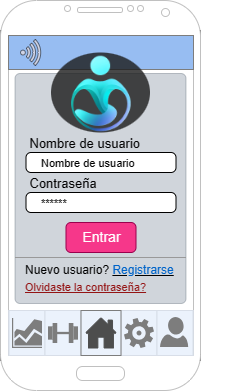
\includegraphics[width=0.35\textwidth]{img/InicioSesion.png}
    \caption{Pantalla de inicio de sesión.}
    \label{fig:inicioSesion} % Esta etiqueta es la que permite que se encuentre referenciada en el texto (es muy importante que siempre estén referenciadas en el texto)
\end{figure}

% ------------------------------------------
% Pantalla de inicio
% Inicio de la figura
\begin{figure}[h]
    \centering
    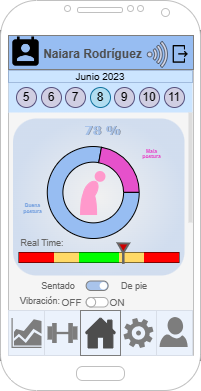
\includegraphics[width=0.33\textwidth]{img/PantallaInicio.png}
    \caption{Pantalla de inicio con información en tiempo real.}
    \label{fig:inicio} % Esta etiqueta es la que permite que se encuentr referenciada en el texto (es muy importante que siempre estén referenciadas en el texto)
\end{figure}

% ------------------------------------------
% Pantalla de estadísticas
% Inicio de la figura
\begin{figure}[h]
    \centering
    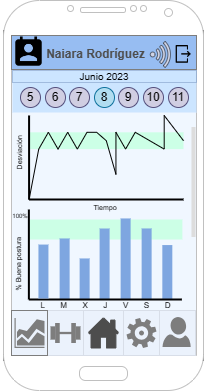
\includegraphics[width=0.33\textwidth]{img/Estadisticas.png}
    \caption{Pantalla con las estadísticas en forma de gráfica de distintos periodos de tiempo.}
    \label{fig:estadisticas} % Esta etiqueta es la que permite que se encuentr referenciada en el texto (es muy importante que siempre estén referenciadas en el texto)
\end{figure}

% ------------------------------------------
% Pantalla de posibles ejercicios y juegos que se puede realizar para mejorar la musculatura y en consecuente mejorar la postura.
% Inicio de la figura
\begin{figure}[h]
    \centering
    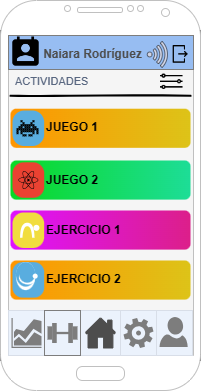
\includegraphics[width=0.33\textwidth]{img/Ejercicios.png}
    \caption{Pantalla con juegos y ejercicios de mejora de la postura.}
    \label{fig:ejercicios} % Esta etiqueta es la que permite que se encuentr referenciada en el texto (es muy importante que siempre estén referenciadas en el texto)
\end{figure}

% ------------------------------------------
% Pantalla de ajustes del dispositivo conectado.
% Inicio de la figura
\begin{figure}[h]
    \centering
    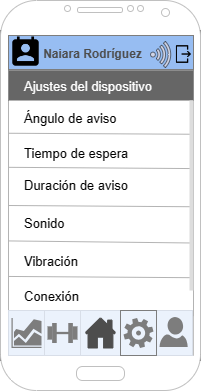
\includegraphics[width=0.33\textwidth]{img/PantallaAjustes.png}
    \caption{Pantalla de ajustes del dispositivo conectado.}
    \label{fig:ajustes} % Esta etiqueta es la que permite que se encuentr referenciada en el texto (es muy importante que siempre estén referenciadas en el texto)
\end{figure}

% ------------------------------------------
% Pantalla de modificación de la información del usuario.
% Inicio de la figura
\begin{figure}[h]
    \centering
    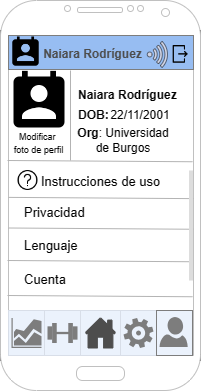
\includegraphics[width=0.33\textwidth]{img/PantallaPerfil.png}
    \caption{Pantalla del perfil del usuario.}
    \label{fig:perfil} % Esta etiqueta es la que permite que se encuentr referenciada en el texto (es muy importante que siempre estén referenciadas en el texto)
\end{figure}

\apendice{Estudio experimental}
Un estudio experimental es una investigación que se realiza con enfoque científico. En estos estudios se pueden medir varias variables y se modifican otras para conocer los diferentes resultados.

En este trabajo no se ha realizado un estudio experimental. Sin embargo, es posible que en el futuro se puedan realizar este tipo de estudios en base al seguimiento de los resultados de diferentes pacientes y la explotación estadística que se puede realizar de los datos recopilados empleando el dispositivo. En el futuro, cuando se obtenga un dispositivo más robusto y avanzado.





% -----------------BIBLIOGRAFÍA-------------------
%\bibliographystyle{plain} % Sin URL con números
%\bibliography{bibliografiaAnexos}

% Si se salen de los márgenes las referencias:
%\newgeometry{left= 3cm, right = 3cm}
\printbibliography[]


\end{document}
